\documentclass[10pt,a4paper]{article}
\usepackage[margin=2cm]{geometry}
\usepackage{graphicx,booktabs,longtable,array,xcolor,amsmath}
\usepackage[colorlinks=true,linkcolor=blue!50!black,urlcolor=blue!50!black]{hyperref}
\usepackage{parskip}
\newcommand{\code}[1]{\texttt{\small #1}}
\newcommand{\neg}[1]{\textcolor{red!70!black}{#1}}
\newcommand{\pos}[1]{\textcolor{green!45!black}{#1}}
\title{\vspace{-1.4cm}CoBit / BitstreamDiffusion --- Research Report\\
\large Friday 4 September -- Tuesday 8 September 2026}
\author{}\date{}
\begin{document}\maketitle\vspace{-1.2cm}

\section*{Summary}
Four workstreams were carried out over five days and 41 commits: the guidance
study was \textbf{closed} with a replication verdict; the error taxonomy was
completed; the \textbf{CE-vs-SM objective} branch was taken through a failed
pilot, a post-mortem, a derivation and a multi-seed stability study; and
\textbf{temporal ordering} was implemented, tested and run to a confirmed
result.

\medskip
\noindent\fbox{\parbox{0.98\textwidth}{%
\textbf{Headline: no intervention tested improved GSM8K accuracy.} Temporal
ordering is neutral at best and harmful at worst. The objective replacement
could not be evaluated for task performance at any budget this environment
permits. Both are clean, well-powered negatives rather than inconclusive runs.
\textbf{The dominant finding is infrastructural}: every training run here
diverges before $\sim$12k steps, while the same code trained 500k steps cleanly
in the collaborator's environment.}}

\section{Research table}
\begin{center}\small
\begin{tabular}{@{}p{2.5cm}p{1.9cm}p{2.1cm}ccccp{2.4cm}p{2.3cm}@{}}
\toprule
\textbf{Experiment} & \textbf{Control} & \textbf{Intervention} & \textbf{Steps} &
\textbf{Seeds} & \textbf{GPU-h} & \textbf{Acc.} & \textbf{$\Delta$ / CI} &
\textbf{Verdict}\\
\midrule
A1 Ordering screen & $w{=}0$ & l2r $w{=}0.1$ & 256 & 1 & 0.65 & 0.1760 &
$+0.0000$ $[-0.020,+0.020]$ & no effect\\
A1 & $w{=}0$ & l2r $w{\geq}0.25$ & 256 & 1 & --- & 0.0000 &
$-0.176$ $[-0.224,-0.132]$ & \neg{collapse}\\
A1 & $w{=}0$ & l2r $w{=}0.25$ & 512 & 1 & --- & 0.0000 &
$-0.184$ $[-0.232,-0.136]$ & \neg{not step-starved}\\
A2 Ordering confirm & $w{=}0$ (0.1387) & \textbf{l2r $w{=}0.1$} & 256 & \textbf{3} &
1.55 & 0.1347 & $-0.0040$, 0/3 sig. & \textbf{no effect}\\
A2 & $w{=}0$ & \textbf{random $w{=}0.1$} & 256 & \textbf{3} & --- & 0.1049 &
$-0.0339$, \textbf{3/3} $p{<}10^{-4}$ & \neg{\textbf{harmful}}\\
B1 Objective & sm @5k & ce @5k & 5k & 1 & 0.16 & 0.000 / 0.000 &
both 250/250 T1 & \neg{unmeasurable}\\
B2 Lift-off & --- & sm/ce @10k & 10k & 1 & 0.06 & 0.0000 & --- &
still zero at 10k\\
B3 Stability & binary\_sm & binary\_ce & 20k & 3+3 & 36.5 & n/a &
rank-sum $p{=}0.05$ & CE $1.80\times$ longer\\
C Prod-era diag. & HEAD & \code{036a2b5} & 20k & 1 & 6.50 & n/a &
broke @11{,}278 & our code exonerated\\
Anchor & --- & production 500k & 500k & 1 & --- & \textbf{0.1640} & --- &
eval pipeline sound\\
\bottomrule
\end{tabular}
\end{center}
\noindent\footnotesize Ordering/objective spend this window $\approx$2.4 GPU-h;
whole-study total $\approx$156 GPU-h. Accuracy on the 1319-problem GSM8K test
set (screens use a fixed 250-problem subset). All comparisons paired, bootstrap
over problems.\normalsize

\section{Temporal ordering (Branch A)}
\textbf{Definition.} Per-token time
$t_j(t)=\mathrm{clip}\!\left(t(1+w)-w\,u_j,\,0,\,1\right)$, with $u_j\in[0,1]$ a
denoising \emph{priority} ($u{=}1$ denoises first) defined over the generated
\textbf{suffix only}. Prompt positions keep the global $\sigma$. At $w{=}0$ every
token gets the global time, i.e.\ today's model --- verified bit-identically.

\textbf{The intervention is causally active}, checked before any GPU spend:
at $w{=}0.5$ the per-position $\sigma$ spread is $192\times$ with the first
suffix token cleanest; at $w{=}1.0$ it is $11{,}247\times$; the prompt stays
pinned at the global value in all cases.

\begin{center}
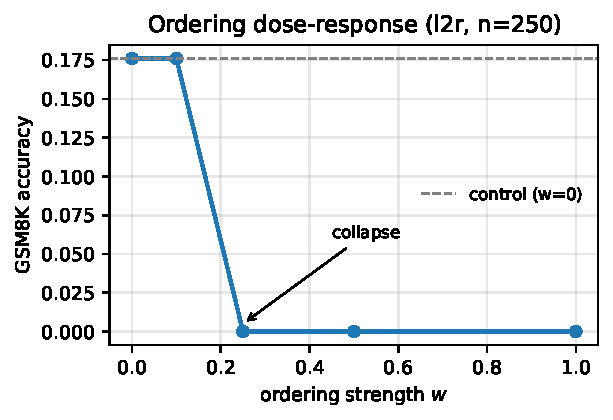
\includegraphics[width=0.48\textwidth]{fig/ordering_dose.pdf}\hfill
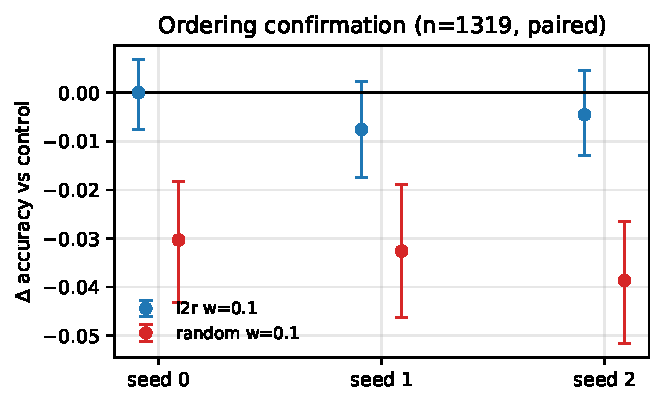
\includegraphics[width=0.50\textwidth]{fig/ordering_confirm.pdf}
\end{center}

\textbf{Result.} At the only strength the model survives ($w{=}0.1$) ordering has
\textbf{no effect} ($-0.0040$, 0/3 seeds significant, CIs $\pm0.008$--$0.017$).
Random ordering is \textbf{reliably harmful} ($-0.0339$, 3/3 seeds,
$p<10^{-4}$). Beyond $w{=}0.25$ the model collapses to zero, and doubling the
trajectory to 512 steps does not rescue it.

\textbf{Interpretation.} The l2r/random asymmetry shows the ordering is doing
something real --- direction matters --- but nothing helps. The model was
\emph{trained} with uniform $\sigma$, so per-position $\sigma$ is
out-of-distribution: it tolerates $\sim$2.9$\times$ spread with no gain and
breaks at $\sim$9$\times$. This does \textbf{not} falsify ordering as a
\emph{training} objective, which is untestable here.

\section{Objective replacement (Branch B)}
The meaningful comparison is \code{binary\_sm} vs \code{binary\_ce}. The
$\sigma$-weighting was \textbf{derived rather than inherited}: matching Bayes-risk
scale gives a factor spanning only $0.250$--$0.361$ across four decades of
$\sigma$ ($0.82$--$1.18\times$ anchored at $\sigma_d$), while gradient-scale
matching is self-defeating because it reintroduces the $D(1{-}D)$ factor under
test. Conclusion: \textbf{no bespoke CE weighting is justified}; both arms use
EDM weighting, clamp off.

\begin{center}

\includegraphics[width=0.49\textwidth]{fig/accuracy_vs_steps.pdf}\hfill
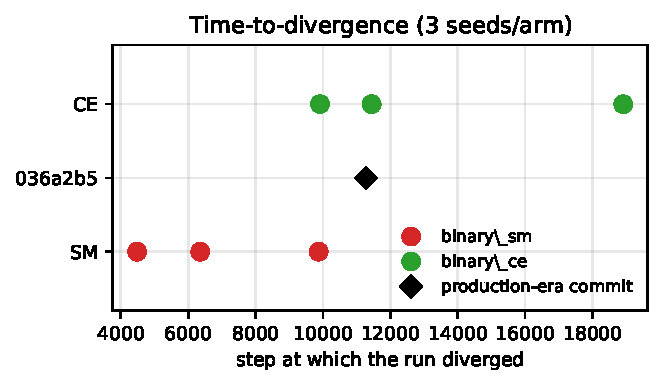
\includegraphics[width=0.49\textwidth]{fig/break_steps.pdf}
\end{center}

\textbf{Task performance: not answerable here.} At a matched 5k steps both arms
score \textbf{exactly 0/250}, with 250/250 non-executing programs and
invalid-token rates differing by 0.001. At 10k both are still 0. The production
anchor scores 0.164 under identical settings, so the evaluation is sound --- the
models are simply nowhere near converged. Accuracy lift-off lies somewhere in
$(10\text{k},\,200\text{k}]$ and is \textbf{unmeasured}.

\textbf{Stability: CE lasts $1.80\times$ longer.} Break steps ---
SM $\{4481, 6356, 9872\}$, CE $\{9911, 11444, 18909\}$ --- perfect rank
separation, exact one-sided rank-sum $p=1/20=0.05$, the floor of a $3{\times}3$
design. \emph{But} the production-era commit broke at 11{,}278, inside the CE
band, so break timing moves more across a numerics-neutral code change than the
effect being measured.

\section{The infrastructural finding}
Seven runs across two code versions diverged before $\sim$12k steps, including
the production-era commit \code{036a2b5} itself. The same code ran 500k steps
with \emph{zero} excursions in the collaborator's environment. Ruled out:
corpus ($\sigma_{\text{data}}$ fingerprint matches to $\sim$8 s.f.), data config
(identical on all 22 keys), and our post-June code changes (fp32
forward+loss+backward \textbf{bit-identical} to the production commit).

Two independent proofs the environments differ: the historical code imports
\code{mauve} at module scope (their env had it, ours does not); and
\code{diffusion/discrete/losses.py} has used PEP 604 in a signature since the
initial release, which \emph{cannot import on Python 3.9} --- so production ran
on $\geq$3.10 while we run 3.9. The production directory is permission-denied,
so their working tree cannot be inspected.

\textbf{Divergence signature}: an abrupt $\sim$400$\times$ jump inside one
20-step interval, with \textbf{no precursor} in gradient norm, logit magnitude,
update RMS or gradient survival; Adam's \code{exp\_avg\_sq} is \emph{declining}
beforehand, then jumps $33\times$. A single-batch loss spike poisons the
optimiser state.

\section{Hypotheses falsified}
\begin{center}\small
\begin{tabular}{@{}p{9cm}p{7.5cm}@{}}
\toprule
\textbf{Hypothesis} & \textbf{Outcome}\\ \midrule
Ordering improves generation & \neg{Falsified} (well-powered null; random worse)\\
CE's advantage appears as retained gradient survival & \neg{Falsified} --- all arms $\sim$0.18 pre-break\\
Low-$\sigma$ weight amplifier causes divergence & \neg{Falsified} by the clamp $2{\times}2$\\
The clamp caused the early break & \neg{Falsified} --- all 6 clamp-off runs diverged\\
Global SM gradient starvation & \neg{Withdrawn} --- survival stable 0.13--0.19\\
Our post-June code caused the divergence & \neg{Falsified} --- prod-era commit diverges too\\
CE is stable & \neg{Falsified} --- the 5k conclusion was an artefact\\
\bottomrule
\end{tabular}
\end{center}

\section{Low-$\sigma$ saturation --- kept separate}
Robust and well measured ($n{=}128$, 2 noise seeds, fully paired): gradient
survival at $\sigma{=}0.05$ falls $0.1475 \to$ \textbf{exactly 0} between 250k
and 500k, with 100.00\% of free bits saturated in \emph{every} evaluation.
Everywhere else training \emph{improves} survival. \textbf{This is descriptive
and causally unlinked} to the divergences, which occur at 4.5k--19k --- nowhere
near a 250k model.

\begin{center}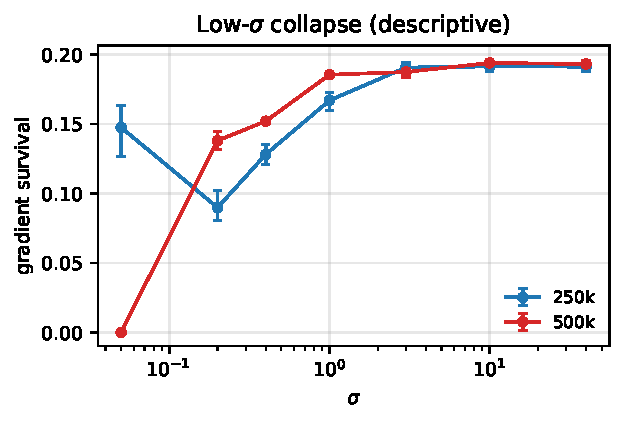
\includegraphics[width=0.52\textwidth]{fig/low_sigma.pdf}\end{center}

\section{Limitations and confounds}
\begin{enumerate}\itemsep2pt
\item \textbf{Environment-limited.} All stability numbers are specific to this
Python 3.9 stack. CE's $1.80\times$ may be an artefact of a broken toolchain
rather than a property of the objectives.
\item \textbf{Ordering was tested at decoding time only}, on a model trained
with uniform $\sigma$. Ordering-as-training remains untested.
\item \textbf{Branch B is budget-blocked, not answered.} Divergence before 12k
and zero accuracy below 10k leave \emph{no window}.
\item $n{=}3$ seeds; $p{=}0.05$ is the design floor.
\item The production working tree is unreadable, so uncommitted differences
cannot be excluded.
\item \textbf{Two of my own bugs invalidated $\sim$1.2 GPU-h}: an over-strict
guidance guard failed 9/9 cells, and the ordering control returned
probabilities from $\sigma_{N-1}$ instead of a final denoise, scoring 0.000
against the baseline's 0.164. The latter was caught only because a production
anchor was included --- without it, seven cells of \emph{confidently wrong}
nulls would have been reported.
\end{enumerate}

\section{Recommendation}
\begin{enumerate}\itemsep2pt
\item \textbf{Close temporal ordering as a decoding intervention.} The result is
well powered and negative. Ordering-as-training is a separate, untested question.
\item \textbf{Fix the environment before any further objective work.} A Python
3.10 environment (\code{sedd310}, torch 2.8.0+cu128) has been built; the
single-variable validation run --- seed 42, the one that broke at 6{,}356 --- is
ready. $\sim$10 GPU-h.
\item \textbf{Do not commit 300+ GPU-h} to a from-scratch CE-vs-SM comparison on
the strength of a $p{=}0.05$ stability difference measured in a suspect
environment. If a performance answer is needed sooner, branch both arms from the
healthy 500k checkpoint ($\sim$25--73 GPU-h), accepting that it answers
``does switching to CE help this model'' rather than ``which objective trains
better''.
\end{enumerate}
\end{document}
